\documentclass[tikz,border=10pt]{standalone}
\usetikzlibrary{arrows.meta, positioning, calc}

\begin{document}
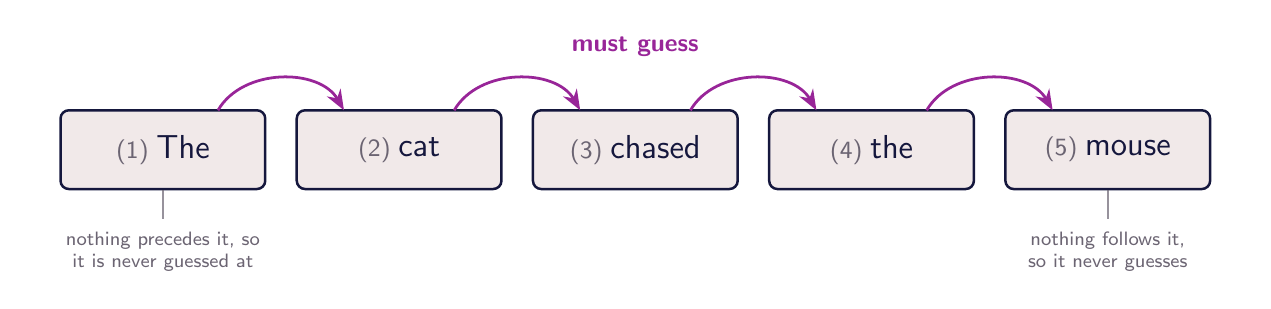
\begin{tikzpicture}[
    every node/.style={font=\sffamily},
]

% ---------------------------------------------------------------- colours
\definecolor{c1}{HTML}{15173D}   % the words, the boxes
\definecolor{c2}{HTML}{982598}   % the guesses (the operative step)
\definecolor{c3}{HTML}{E491C9}
\definecolor{c4}{HTML}{F1E9E9}
\definecolor{axiscolor}{HTML}{333333}
\definecolor{labelcolor}{HTML}{6B6472}

% ================================================================
% Geometry, decided before any TikZ was written.
%
%   five word boxes, one row, y = 0, height 1.0 (top +0.5, bottom -0.5)
%   box width 2.6, pitch 3.0  ->  gap 0.4
%   centres  x = 0, 3, 6, 9, 12
%
%   four arcs above the strip: from (x_i + 0.7, 0.5) to (x_{i+1} - 0.7, 0.5)
%   span 1.6, bend left 60  ->  apex about y = 0.95
%   shared label "must guess" sits at (6, 1.06), in the dip between arcs 2 and 3
%
%   annotations below: ticks drop from box (1) and box (5) to y = -0.85,
%   text blocks 3.2cm wide, centred under (1) and under (5),
%   so each stays inside its own box's column and they cannot collide
%
%   bounding box roughly x in [-1.4, 13.4], y in [-2.1, 1.9]: wide and short
% ================================================================

\def\pitch{3.0}

\tikzset{
    wordbox/.style={
        draw=c1, line width=0.9pt, fill=c4,
        rounded corners=3pt,
        minimum width=2.6cm, minimum height=1.0cm,
        inner sep=0pt,
    },
    guess/.style={
        draw=c2, line width=1.0pt,
        -{Stealth[length=2.6mm, width=2.0mm]},
    },
    tick/.style={draw=labelcolor, line width=0.6pt, opacity=0.7},
    note/.style={font=\sffamily\scriptsize, text=labelcolor,
        text width=3.2cm, align=center},
}

% ---------------------------------------------------------------- the strip
\foreach \i/\w in {0/The, 1/cat, 2/chased, 3/the, 4/mouse} {
    \pgfmathsetmacro{\x}{\i*\pitch}
    \pgfmathtruncatemacro{\p}{\i+1}
    \node[wordbox] (b\p) at (\x, 0)
        {{\small\textcolor{labelcolor}{(\p)}}\;{\large\textcolor{c1}{\w}}};
}

% ---------------------------------------------------------------- the guesses
\foreach \i in {1,2,3,4} {
    \pgfmathsetmacro{\xa}{(\i-1)*\pitch + 0.7}
    \pgfmathsetmacro{\xb}{\i*\pitch - 0.7}
    \draw[guess] (\xa, 0.5) to[bend left=60] (\xb, 0.5);
}

\node[font=\sffamily\small\bfseries, text=c2, anchor=south] at (6, 1.06)
    {must guess};

% ---------------------------------------------------------------- annotations
\draw[tick] (b1.south) -- (0, -0.88);
\draw[tick] (b5.south) -- (12, -0.88);

\node[note, anchor=north] at (0, -0.92)
    {nothing precedes it, so it is never guessed at};
\node[note, anchor=north] at (12, -0.92)
    {nothing follows it, so it never guesses};

\end{tikzpicture}
\end{document}
